\documentclass[tikz,border=2pt]{standalone}
\usepackage{amsmath}
\usetikzlibrary{arrows.meta,positioning,calc}

\begin{document}
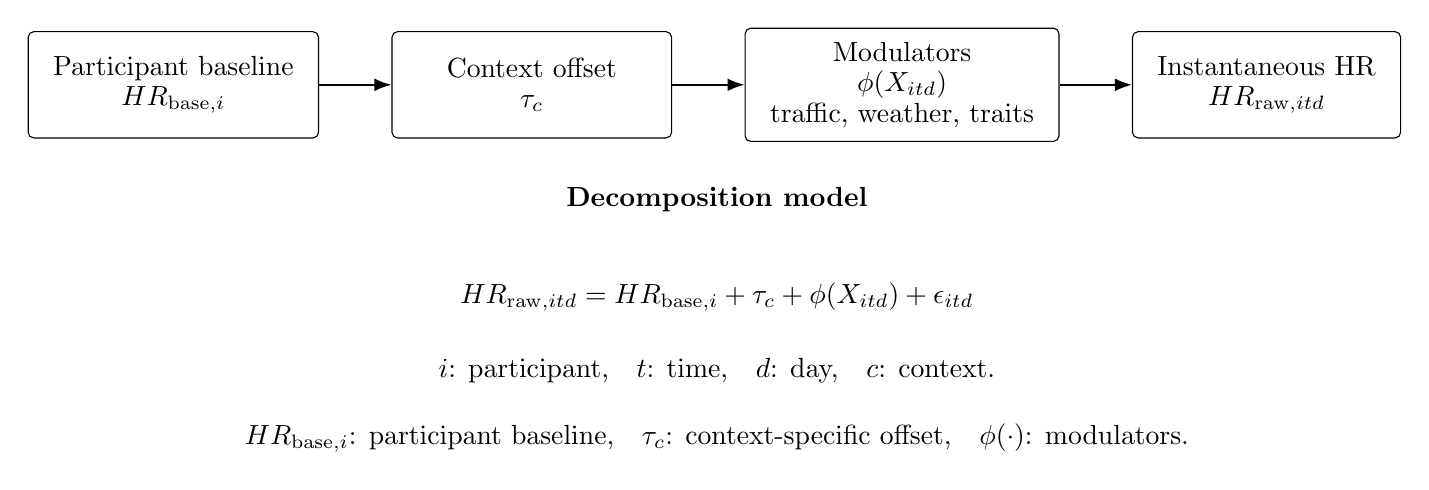
\begin{tikzpicture}[
  font=\normalsize,
  >=Latex,
  node distance=0.92cm,
  box/.style={
    draw,
    rounded corners=2pt,
    minimum height=1.35cm,
    align=center,
    inner xsep=9pt,
    inner ysep=5pt
  },
  arrow/.style={->, line width=0.7pt}
]

\node[box, minimum width=3.15cm] (baseline) {
  Participant baseline\\[-1pt]
  $HR_{\mathrm{base},i}$
};

\node[box, minimum width=3.55cm, right=of baseline] (offset) {
  Context offset\\[-1pt]
  $\tau_c$
};

\node[box, minimum width=3.75cm, right=of offset] (mods) {
  Modulators\\[-1pt]
  $\phi(X_{itd})$\\[-1pt]
  traffic, weather, traits
};

\node[box, minimum width=3.20cm, right=of mods] (hr) {
  Instantaneous HR\\[-1pt]
  $HR_{\mathrm{raw},itd}$
};

\draw[arrow] (baseline) -- (offset);
\draw[arrow] (offset) -- (mods);
\draw[arrow] (mods) -- (hr);

\node[below=1.18cm of $(offset)!0.5!(mods)$, font=\bfseries] (title) {Decomposition model};

\node[below=0.65cm of title] (eq) {
  $HR_{\mathrm{raw},itd}=HR_{\mathrm{base},i}+\tau_c+\phi(X_{itd})+\epsilon_{itd}$
};

\node[below=0.34cm of eq] (indices) {
  $i$: participant,\quad $t$: time,\quad $d$: day,\quad $c$: context.
};

\node[below=0.28cm of indices] (defs) {
  $HR_{\mathrm{base},i}$: participant baseline,\quad
  $\tau_c$: context-specific offset,\quad
  $\phi(\cdot)$: modulators.
};

\end{tikzpicture}
\end{document}
